\chapter{Programmation linéaire}

\section{Introduction}

Bien que la réalité soit souvent loin d'être linéaire, un grand nombre de problèmes peuvent s'écrire sous forme linéaire, soit directement, soit en première simplification.
D'autre part, un très grand nombre de modèles constituent des extensions de programmes linéaires. Sa compréhension est essentielle à la compréhension de modèles plus sophistiqués.

Un programme linéaire générique s'écrit sous la forme
\[
\begin{matrix}
\max_x & c_1x_1 & + & \ldots & + & c_n x_n \\
& a_{11}x_1 & + & \ldots & + & a_{1n} x_n & \leq b_1 \\
& \vdots & & & \vdots \\
& a_{m1}x_1 & + & \ldots & + & a_{mn} x_n & \leq b_m,
\end{matrix}
\]
ou, sous une forme plus compacte,
\begin{align*}
\max_x & \sum_{j = 1}^n c_jx_j \\
& \sum_{j = 1}^n a_{ij}x_j \leq b_i, \quad i = 1,\ldots,m.
\end{align*}
La ligne
\[
\sum_{j = 1}^n c_jx_j
\]
représente la {\sl fonction objectif}, que nous souhaitons maximiser.
La maximisation se fait en respectant les $m$ {\sl contraintes}
\[
\sum_{j = 1}^n a_{ij}x_j \leq b_i, \quad i = 1,\ldots,m.
\]

Sous forme matricielle, le problème se réecrit
\begin{align*}
\max_x\ & c^T x \\
& Ax \leq b,
\end{align*}
avec
\begin{align*}
x &= \begin{pmatrix} x_1 \\ \vdots \\ x_n \end{pmatrix}, \quad
c = \begin{pmatrix} c_1 \\ \vdots \\ c_n \end{pmatrix}, \quad
b = \begin{pmatrix} b_1 \\ \vdots \\ b_n \end{pmatrix} \\
A &= \begin{pmatrix}
a_{11} & a_{12} & \ldots & a_{1n} \\
a_{21} & a_{22} & \ldots & a_{2n} \\
a_{m1} & a_{m2} & \ldots & a_{mn}
\end{pmatrix}.
\end{align*}

La terminologie ``linéaire'' vient du fait que toutes les fonctions impliquées sont linéaires.
Typiquement, nous ajouterons également des contraintes de non-négativités:
\[
x_i \geq 0,\ i = 1,\ldots,n,
\]
ou, en abrégé,
\[
x \geq 0.
\]
Nous dirons aussi que le vecteur $x$ appartient à l'orthant positif (i.e. $x \in \RR_+^n$).

\begin{example}[Wyndor Glass]
\label{ex:wyndor}
La compagnie Wyndor Glass Co. produit des produits verriers de haute qualité, incluant des fenêtres et des portes vitrées.
Elle dispose à cette fin de trois usines (usine 1, usine 2, usine 3), qui ont chacune une capacité de production limitée.
Les châssis en aluminium et les matériaux sont produits dans l'usine 1, les châssis en bois sont fabriqués dans l'usine 2, et l'usine 3 produit le verre et assemble les produits.
La compagnie a décidé de mettre en place de ligne de production:
\begin{itemize}
\item
produit 1: une porte vitrée avec un châssis d'aluminium;
\item
produit 2: une fenêtre double-vitrage avec châssis en bois.
\end{itemize}

Un lot de 20 unités donne lieu à un profit de \$3000 et \$5000, respectivement pour le produit 1 et le produit 2. Les données du problème sont synthétisées dans la Table~\ref{tab:wyndor}.
\begin{table}[htbp]
\begin{center}
\begin{tabular}{|c|c|c|c|}
\hline
& Produit 1 & Produit 2 & Capacité de \\
& Temps de prod. (h) & Temps de prod. (h)& production (h)\\
\hline
Usine 1 & 1 & 0 & 4 \\
\hline
Usine 2 & 0 & 2 & 12 \\
\hline
Usine 3 & 3 & 2 & 18 \\
\hline
\end{tabular}
\end{center}
\caption{Données du problème Wyndor Glass}
\label{tab:wyndor}
\end{table}
Chaque lot d'un produit est le résultat combiné de la production dans les trois usines.
Nous souhaitons déterminer le taux de production pour chaque produit (nombre de lots par semaine) de façon à maximiser le profit total.

Les variables de décision sont
\begin{itemize}
\item
$x_1$, le nombre de lots du produit 1;
\item
$x_2$, le nombre de lots du produit 2.
\end{itemize}
Le fonction objectif est le profit total, qui vaut $3x_1 +5x_2$, en l'exprimant en miller de dollars. Nous voulons maximiser ce profit.

Les contraintes concernent tout d'abord les capacítés de production:
\begin{eqnarray*}
x_1 & \leq 4 & \mbox{(usine 1)} \\
2x_2 & \leq 12 & \mbox{(usine 2)} \\
3x_1 + 2x_2 & \leq 18  & \mbox{(usine 3)}
\end{eqnarray*}
Viennent ensuite les contriantes de non-négativité:
\[
x_1 \geq 0, x_2 \geq 0. \qquad \mbox{(nombre positif d'unités produites)}
\]

En résumé, nous avons le problème d'optimisation suivant:
\[
\max_x z = 3x_1 + 5x_2
\]
sous les contraintes
\begin{eqnarray*}
x_1\qquad & \leq 4 & \mbox{(usine 1)} \\
 \qquad  2x_2 & \leq 12 & \mbox{(usine 3)} \\
3x_1 + 2x_2 & \leq 18 & \mbox{(usine 3)}
\end{eqnarray*}
\[
x_1 \geq 0,\ x_2 \geq 0\ \mbox{(non-négativité)}
\]

Avant de traiter de méthodes numériques, essayons de visualiser le problème afin de développer une intuition quand à sa résolution.
Le problème peut-être représenté comme sur la Figure~\ref{fig:wyndor}.
Pour le réaliser, nous traçons d'abord les droites correpondant aux contraintes, puis nous déterminons le domaine réalisable en vérifiant le sens des inégalités pour chacune d'elle.
Nous traçons ensuite les droites correspondant à la variation de l'objectif.
Dans l'exemple
\[
z = 3x_1+5x_2 \Leftrightarrow x_2 = -\frac{3}{5}x_1 + \frac{1}{5}z.
\]
L'ordonnée à l'origine, dépendant de la valeur de $z$, est $\frac{1}{5}z$, et la pente vaut $-\frac{3}{5}$.
Maximiser revient à augmenter $z$.
\begin{figure}[htbp]
\begin{center}
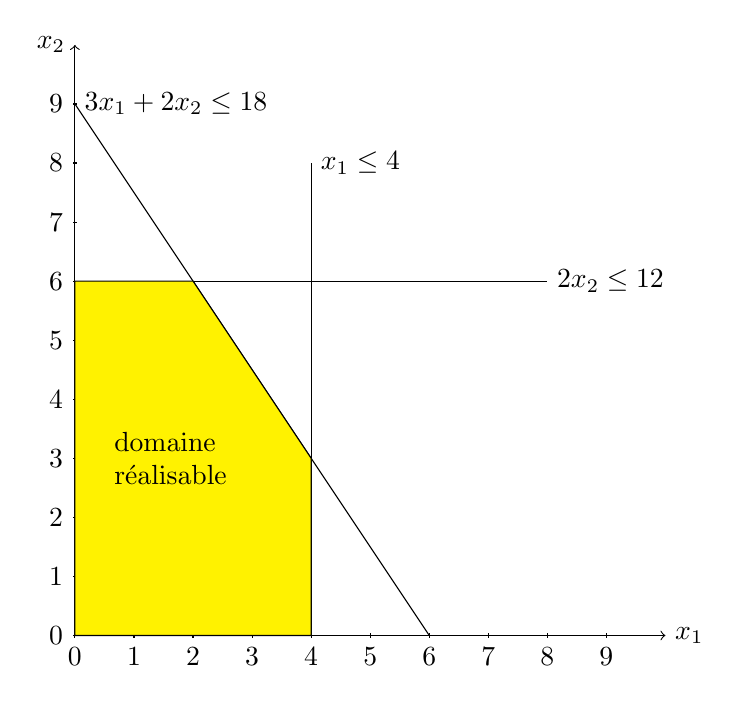
\begin{tikzpicture}[scale=0.75]
\draw[->] (0,0) -- (10,0) node[below,right] {$x_1$};
\draw[->] (0,0) -- (0,10) node[above,left] {$x_2$};
\draw (6,0) -- (0,9) node[above,right] {$3x_1 + 2x_2 \leq 18$};
\draw (0,6) -- (8,6) node[right] {$2x_2 \leq 12$};
\draw (4,0) -- (4,8) node[above,right] {$x_1 \leq 4$};

\foreach \x in {0,1,2,3,4,5,6,7,8,9}
  \draw (\x,1pt) -- (\x,-1pt) node[anchor=north] {$\x$};
\foreach \y in {0,1,2,3,4,5,6,7,8,9}
  \draw (1pt,\y) -- (-1pt,\y) node[anchor=east] {$\y$};

\filldraw[fill=yellow]
  (0,0) -- (0,6) -- (2,6) -- (4,3) -- (4,0) -- (0,0);
  
\draw (2,3) node[text width=2cm,text ragged] {domaine réalisable};

\end{tikzpicture}
\end{center}
\caption{exemple Wyndor Glass}
\label{fig:wyndor}
\end{figure}

\begin{figure}[htbp]
\begin{center}
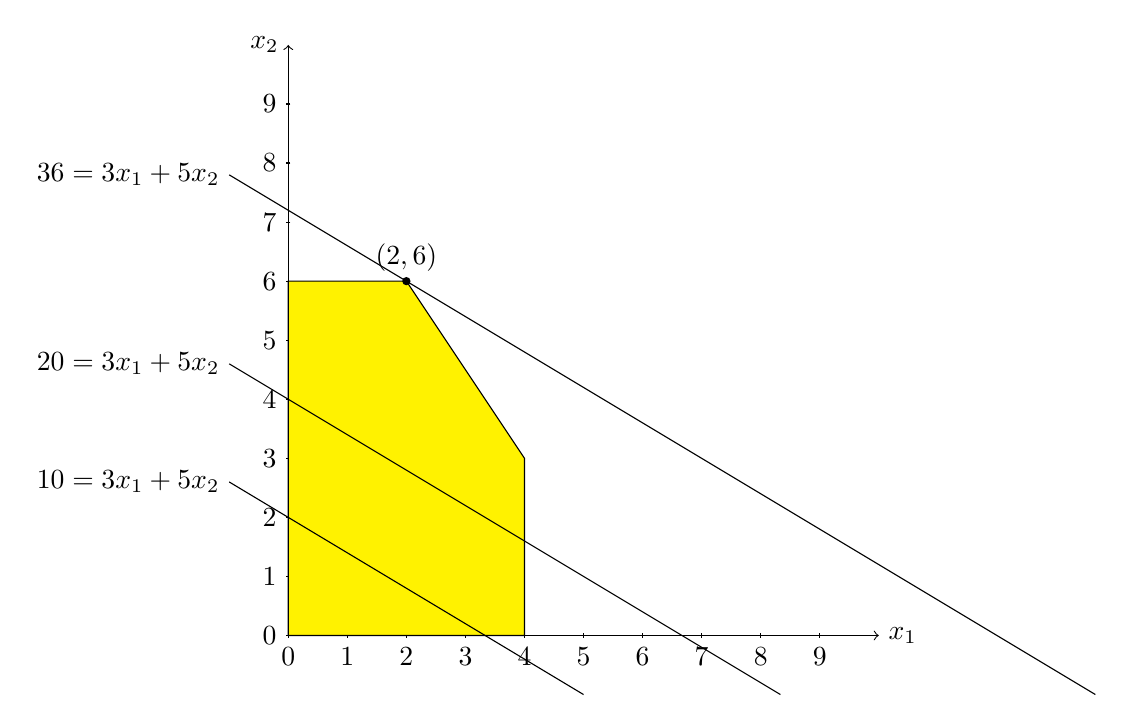
\begin{tikzpicture}[scale=0.75]
\draw[->] (0,0) -- (10,0) node[below,right] {$x_1$};
\draw[->] (0,0) -- (0,10) node[above,left] {$x_2$};

\foreach \x in {0,1,2,3,4,5,6,7,8,9}
  \draw (\x,1pt) -- (\x,-1pt) node[anchor=north] {$\x$};
\foreach \y in {0,1,2,3,4,5,6,7,8,9}
  \draw (1pt,\y) -- (-1pt,\y) node[anchor=east] {$\y$};

\filldraw[fill=yellow]
  (0,0) -- (0,6) -- (2,6) -- (4,3) -- (4,0) -- (0,0);

\draw (5.0,-1) -- (-1,13.0/5) node[above,left] {$10=3x_1+5x_2$};
\draw (25.0/3,-1) -- (-1,23.0/5) node[above,left] {$20=3x_1+5x_2$};
\draw (41.0/3,-1) -- (-1,39.0/5) node[above,left] {$36=3x_1+5x_2$};

\draw (2,6) node[above] {$(2,6)$};
\fill (2,6) circle (2 pt);

\end{tikzpicture}
\end{center}
\caption{exemple Wyndor Glass: maximisation}
\label{fig:wyndor_2}
\end{figure}
\end{example}

La représentation graphique, bien qu'intéressante pour ``voir'' comment se passe les choses, ne fonctionnent plus dès que nous avons plus de deux variables.
Il faut alors passer à l'utilisation de logiciels, utilisant l'algorithme du simplexe ou de points intérieurs.
Nous n'aborderons que le premier dans le cadre de ce cours introductif.

\section{Modèle général de programmation linéaire}

Le modèle complet
\begin{align*}
\max_x\ & c^T x \\
& Ax \leq b, \\
& x \geq 0,
\end{align*}
est appelé {\sl forme standard}.
Le modèle complet
\begin{align*}
\max_x\ & c^T x \\
& Ax \leq b, \\
& x \geq 0,
\end{align*}
est appelé {\sl forme standard}.

D'autres formes sont possibles et définissent aussi des modèles de programmation linéaire:
\begin{itemize}
\item
minimiser au lieu de maximiser:
\[
\min f(x) = -\max f(x);
\]
\item
les inégalités peuvent être remplacées par des égalités, ou être de sens contraire;
\item
certaines variables peuvent ne pas être forcés à être supérieures à 0. Par exemple, considérons la contrainte
\[
x \geq -4,
\]
qui équivaut à
\[
x + 4 \geq 0.
\]
Nous pouvons alors définir $y = x+4$, de sorte que la contrainte devient
\[
y \geq 0.
\]
De même, considérons
\[
-10 \leq x \leq -2.
\]
En définissons $y = x+10$, nous avons la contrainte $y \geq 0$.
\end{itemize}

\section{Terminologie de base}

Nous parlerons de {\sl solution réalisable} à propos d'une solution (i.e. une instance particulière du vecteur $x$) pour laquelle toutes les contraintes sont satisfaites.
En d'autres termes cette solution appartient au domaine réalisable.
Par exemple, le point $(1,1)$ est une solution réalisable pour la Figure~\ref{fig:wyndor}.
A contrario, une solution non réalisable est une solution pour laquelle au moins une contrainte est violée. Elle n'appartient pas au domaine réalisable.
Une {\sl solution optimale} est une solution donnant la meilleure valeur possible pour l'objectif. Cette valeur est dite {\sl valeur optimale}.
Un modèle n'a aucune solution optimale si son domaine réalisable est vide, ou si la fonction objectif est non bornée.
Ajoutons par exemple la contrainte
\[
3x_1 + 5x_2 \geq 50
\]
dans l'exemple Wyndor Glass.
Cette nouvelle contrainte ne peut être satisfaite en même temps que les contraintes précédentes, comme illustré dans la Figure~\ref{fig:wyndor_unfeasible}.
Plus aucun point n'est réalisable.
Si nous supprimons plutôt les contraintes
\[
2x_2 \geq 12,\quad 3x_1 + 2x_2 \leq 18,
\]
la fonction objectif devient non bornée dans le domaine réalisable, comme illustré sur la Figure~\ref{fig:wyndor_unbounded}.
Un modèle peut également présenter une infinité de solutions optimales.
Considérons dans l'exemple la fonction objectif
\[
z = 3x_1 + 2x_2.
\]
Tout point sur le segment $[(2,6),(4,3)]$ est alors solution optimale (voir Figure~\ref{fig:wyndor_infinite}).

\begin{figure}[htbp]
\begin{center}
\begin{tikzpicture}[scale=0.75]
\draw[->] (0,0) -- (10,0) node[below,right] {$x_1$};
\draw[->] (0,0) -- (0,11) node[above,left] {$x_2$};

\draw[->] (1,6) -- (1,5.5);
\draw[->] (2,0) -- (2,0.5);
\draw[->] (0,3) -- (0.5,3);
\draw[->] (4,1.5) -- (3.5,1.5);
\draw[->] (3,4.5) -- (2.584,4.223);
\draw[->] (5,7) -- (5.257,7.429);

\foreach \x in {0,1,2,3,4,5,6,7,8,9}
  \draw (\x,1pt) -- (\x,-1pt) node[anchor=north] {$\x$};
\foreach \y in {0,1,2,3,4,5,6,7,8,9,10}
  \draw (1pt,\y) -- (-1pt,\y) node[anchor=east] {$\y$};

\draw
  (0,0) -- (0,6) -- (2,6) -- (4,3) -- (4,0) -- (0,0);

\draw (0,10) -- (10,4);

\end{tikzpicture}
\end{center}
\caption{exemple Wyndor Glass: domaine non réalisable}
\label{fig:wyndor_unfeasible}
\end{figure}

\begin{figure}[htbp]
\begin{center}
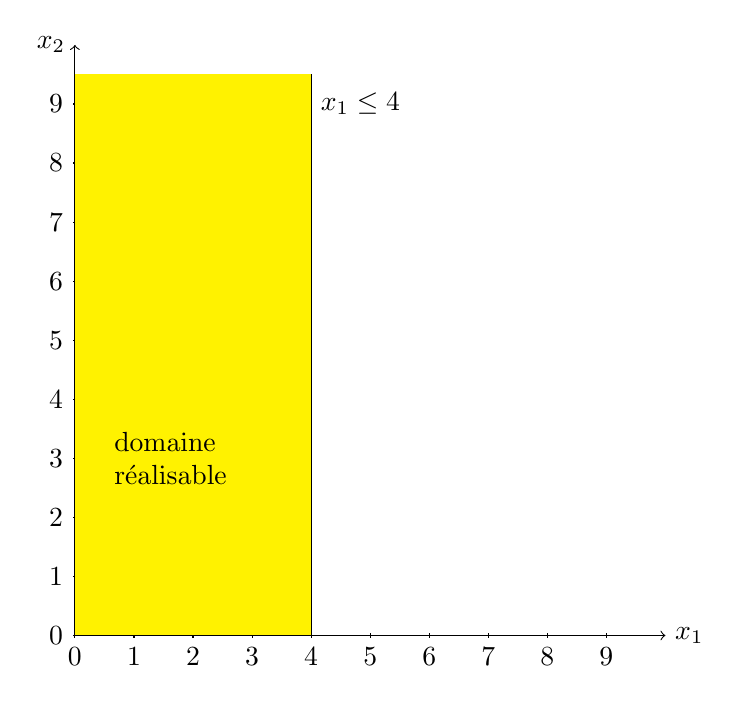
\begin{tikzpicture}[scale=0.75]
\draw[->] (0,0) -- (10,0) node[below,right] {$x_1$};
\draw[->] (0,0) -- (0,10) node[above,left] {$x_2$};
\draw (4,0) -- (4,9) node[above,right] {$x_1 \leq 4$};

\foreach \x in {0,1,2,3,4,5,6,7,8,9}
  \draw (\x,1pt) -- (\x,-1pt) node[anchor=north] {$\x$};
\foreach \y in {0,1,2,3,4,5,6,7,8,9}
  \draw (1pt,\y) -- (-1pt,\y) node[anchor=east] {$\y$};

\filldraw[fill=yellow]
  (0,0) -- (0,9.5) -- (4,9.5) -- (4,0) -- (0,0);
 \draw[color=yellow] (0,9.5) -- (4,9.5);
  
 \draw (2,3) node[text width=2cm,text ragged] {domaine réalisable};

\end{tikzpicture}
\end{center}
\caption{exemple Wyndor Glass: objectif non borné}
\label{fig:wyndor_unbounded}
\end{figure}

\begin{figure}[htbp]
\begin{center}
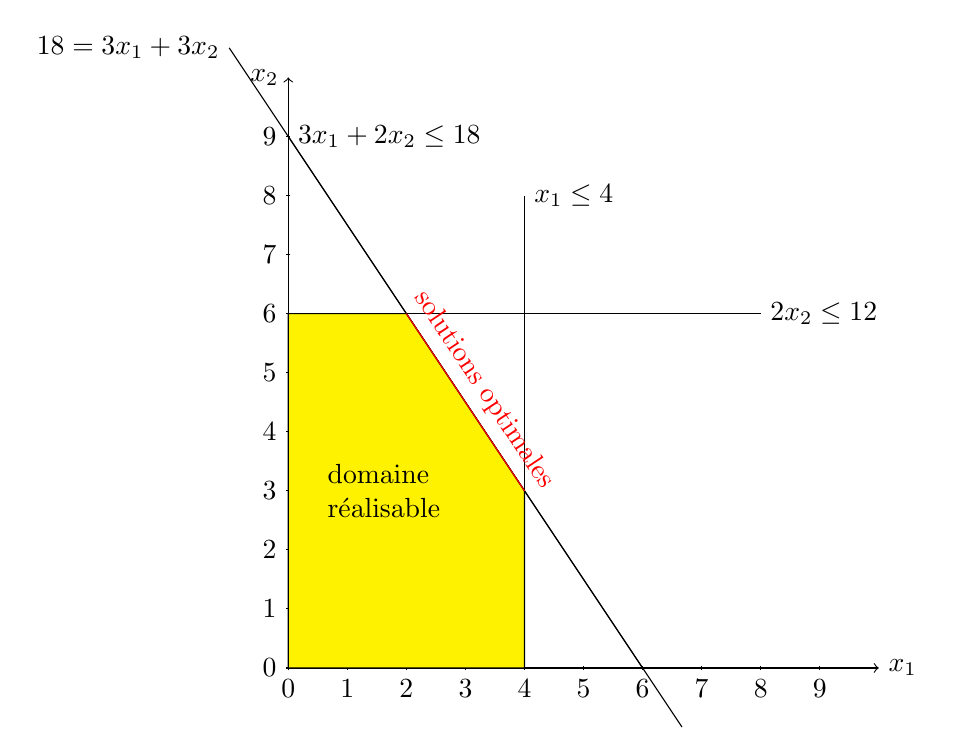
\begin{tikzpicture}[scale=0.75]
\draw[->] (0,0) -- (10,0) node[below,right] {$x_1$};
\draw[->] (0,0) -- (0,10) node[above,left] {$x_2$};
\draw (6,0) -- (0,9) node[above,right] {$3x_1 + 2x_2 \leq 18$};
\draw (0,6) -- (8,6) node[right] {$2x_2 \leq 12$};
\draw (4,0) -- (4,8) node[above,right] {$x_1 \leq 4$};

\foreach \x in {0,1,2,3,4,5,6,7,8,9}
  \draw (\x,1pt) -- (\x,-1pt) node[anchor=north] {$\x$};
\foreach \y in {0,1,2,3,4,5,6,7,8,9}
  \draw (1pt,\y) -- (-1pt,\y) node[anchor=east] {$\y$};

\filldraw[fill=yellow]
  (0,0) -- (0,6) -- (2,6) -- (4,3) -- (4,0) -- (0,0);
  
 \draw (2,3) node[text width=2cm,text ragged] {domaine réalisable};

\draw (20.0/3,-1) -- (-1,10.5) node[above,left] {$18=3x_1+3x_2$};

\draw[color=red] (2,6)--(4,3) node[midway,above,sloped] {solutions optimales};

\end{tikzpicture}
\end{center}
\caption{exemple Wyndor Glass: infinité de solutions}
\label{fig:wyndor_infinite}
\end{figure}

\section{Hypothèses}

La première hypothèse d'un modèle de programmation linéaire est la {\sl proportionnalité}:
\begin{itemize}
\item
la contribution de chaque variable à la valeur de la fonction objectif est proportionnelle à la valeur de cette variable.
\item
la contribution de chaque variable au terme de gauche de chaque contrainte fonctionnelle est proportionnelle à la valeur de cette variable.
\end{itemize}
Des cas où cette hypothèse n'est pas satisfaite sont
\begin{itemize}
\item
coût fixe initial (Figure~\ref{fig:initial_cost}).
\item
profit marginal (profit par unité) croissant ou décroissant (Figure~\ref{fig:profit}).
\end{itemize}
\begin{figure}[htbp]
\begin{center}
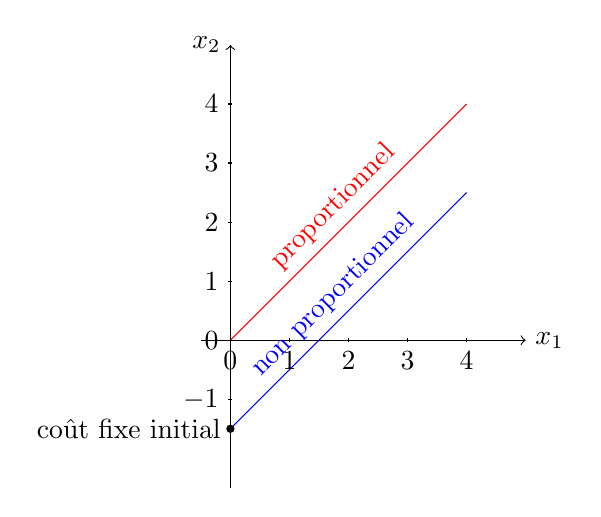
\begin{tikzpicture}[scale=0.75]
\draw[->] (-0.5,0) -- (5,0) node[below,right] {$x_1$};
\draw[->] (0,-2.5) -- (0,5) node[above,left] {$x_2$};
\draw[red] (0,0) -- (4,4) node[sloped,midway,above] {proportionnel};
\draw[blue] (0,-1.5) -- (4,2.5) node[sloped,midway,above] {non proportionnel};
\draw (0,-1.5) node[left] {coût fixe initial};

\fill (0,-1.5) circle (2 pt);

\foreach \x in {0,1,2,3,4}
  \draw (\x,1pt) -- (\x,-1pt) node[anchor=north] {$\x$};
\foreach \y in {-1,0,1,2,3,4}
  \draw (1pt,\y) -- (-1pt,\y) node[anchor=east] {$\y$};

\end{tikzpicture}
\end{center}
\caption{coût fixe initial}
\label{fig:initial_cost}
\end{figure}

\begin{figure}[htbp]
\begin{center}
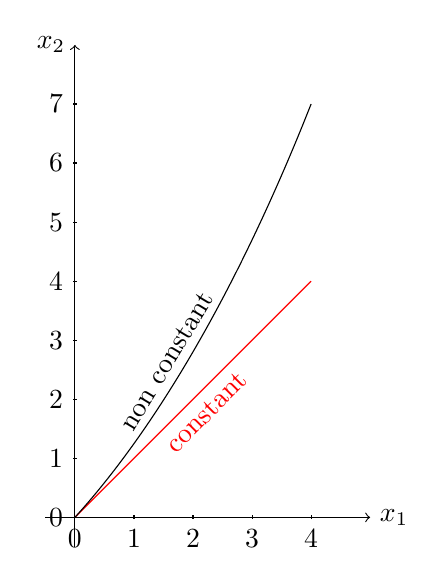
\begin{tikzpicture}[scale=0.75]
\draw[->] (-0.5,0) -- (5,0) node[below,right] {$x_1$};
\draw[->] (0,-0.5) -- (0,8) node[above,left] {$x_2$};
\draw[red] (0,0) -- (4,4) node[sloped,midway,below] {constant};
\draw (0,0) .. controls (1,1.1) and (2.5,3.2) ..  node[sloped, above] {non constant} (4,7);

\foreach \x in {0,1,2,3,4}
  \draw (\x,1pt) -- (\x,-1pt) node[anchor=north] {$\x$};
\foreach \y in {0,1,2,3,4,5,6,7}
  \draw (1pt,\y) -- (-1pt,\y) node[anchor=east] {$\y$};

\end{tikzpicture}
\end{center}
\caption{profit marginal}
\label{fig:profit}
\end{figure}
Nous avons d'autre part la propriété d'additivité: la fonction objectif est composée de la somme des contributions individuelles de chaque variable, et le terme de gauche de chaque contrainte fonctionnelle est composé de la somme des contributions individuelles de chaque variable.
L'additivité interdit les termes de la forme $x_1x_2$.
Si une de ces hypothèses est invalidée, nous sommes en présence d'un programme non linéaire, étudié au Chapitre~\ref{chap:nonlinear}.

D'autre part, les variables sont continues. Si nous imposons des variables à valeurs entières, nous obtenons un modèle de programmation en nombres entiers (Chapitre~\ref{chap:integer}).
De plus, les valeurs affectées à chaque paramètre sont des constantes connues avec certitude.
Cette hypothèse peut être fort éloignée de la réalité.
Nous pouvons tester cette hypothèse en conduisant une {\sl analyse de sensibilité}, qui consiste à vérifier la sensibilité du modèle à des changements de valeurs des paramètres.
Nous pouvons également introduire des variables aléatoires, ce qui conduit typiquement à un problème de programmation stochastique.
La programmation stochastique dépasse cependant les objectifs du présent cours.

\begin{example}[Horaire de personnel]
Nous souhaitons établir un horaire quotidien, sachant que chaque jour est divisé en périodes et en supposant que nous avons pu estimer un nombre minimum d'employés devant être affecté durant chaque période.
Chaque jour est divisé en quarts de travail de 8 heures. Plusieurs quarts partagent une même période, mais chaque quart exige un salaire particulier.
Nous souhaitons savoir combien d'employés doit-on affecter à chaque quart de travail de façon à minimiser le total des salaires versés, en respectant le nombre minimum d'employés pour chaque période. Les données du problème sont données dans la Table~\ref{tab:horaire}.

\begin{table}[htbp]
\begin{center}
\begin{tabular}{|c|c|c|c|c|c|c|}
\hline
Période & Quart 1 & Quart 2 & Quart 3 & Quart 4 & Quart 5 & Minimum employés \\
\hline
6--8 & X & & & & & 48 \\
\hline
8--10 & X & X & & & & 79 \\
\hline
10--12 & X & X & & & & 65 \\
\hline
12--14 & X & X & X & & & 87 \\
\hline
14--16 & & X & X & & & 64 \\
\hline
16--18 & & & X & X & & 73 \\
\hline
18--20 & & & X & X & & 82 \\
\hline
20--22 & & & & X & & 43 \\
\hline
22--24 & & & & X & X & 52 \\
\hline
0--6 & & & & & X & 15 \\
\hline
Salaire & 170 & 160 & 175 & 180 & 195 & \\
\hline
\end{tabular}
\caption{données du problème d'horaire de personnel}
\label{tab:horaire}
\end{center}
\end{table}

Comme variables, nous pouvons choisir $x_j$ comme le nombre d'employés affectés au quart $j$.
L'objectif est
\[
\min z = 170 x_1 + 160 x_2 + 175 x_3 + 180 x_4 + 195 x_5.
\]
Pour chaque période, le nombre d'employés affectés aux différents quarts doit couvrir le minimum d'employés requis pour cette période. Par exemple, pour la période de 14h à 16h, nous aurons:
\[
x_2+x_3 \geq 64.
\]

Le programme linéaire résultant est
\begin{align*}
\min z \ & = 170 x_1 + 160 x_2 + 175 x_3 + 180 x_4 + 195 x_5, \\
\mbox{s.c. } & x_1 \geq 48, \\
& x_1 + x_2 \geq 79 \\
& x_1 + x_2 \geq 65 \\
& x_1 + x_2 + x_3 \geq 87 \\
& x_2 + x_3 \geq 64 \\
& x_3 + x_4 \geq 73 \\
& x_3 + x_4 \geq 82 \\
& x_4 \geq 43 \\
& x_4 + x_5 \geq 52 \\
& x_5 \geq 15 \\
& x_j \geq 0,\ j = 1,2,3,4,5.
\end{align*}

Nous pouvons remarquer la présence de contraintes redondantes:
\begin{itemize}
\item
si nous avons $x_1 + x_2 \geq 79$, alors $x_1 + x_2 \geq 65$; cette dernière contrainte est donc {\sl redondante} et peut être éliminée;
\item
de même, $x_3 + x_4 \geq 82$ implique $x_3 + x_4 \geq 73$;
\item
les contraintes $x_1 \geq 0$, $x_4 \geq 0$, $x_5 \geq 0$, sont aussi redondantes, mais il n'y a aucun intérêt à les éliminer.
\end{itemize}
La solution optimale du problème est
\[
\bx^* = (x^*_1, x^*_2, x^*_3, x^*_4, x^*_5) = (48, 31, 39, 43, 15).
\]
Une difficulté est que le nombre d'employés doit toujours être entier, aussi l'hypothèse de continuité n'est pas satisfaite dans le modèle (bien que la solution optimale dans ce cas particulier soit entière).
\end{example}

\begin{example}[Réseau de distribution]
\label{ex:distribution}

Considérons deux usines ($U1$ et $U2$), un centre de distribution ($CD$), et deux entrepôts ($E1$, $E2$).
Chaque usine manufacture un certain nombre d'unités d'un même produit (offre).
Chaque entrepôt requiert un certain nombre d'unités de ce même produit (demande).
Sur chaque lien (arc) du réseau, il y a un coût de transport par unité de produit (coût unitaire).
De plus, sur certains arcs, il y a une capactité sur le nombre d'unités transportées.
Le réseau considéré est représenté dans la Figure~\ref{fig:network_linear}.
L'objectif est de minimiser le coût de transport total.

\begin{figure}[htbp]
\begin{center}
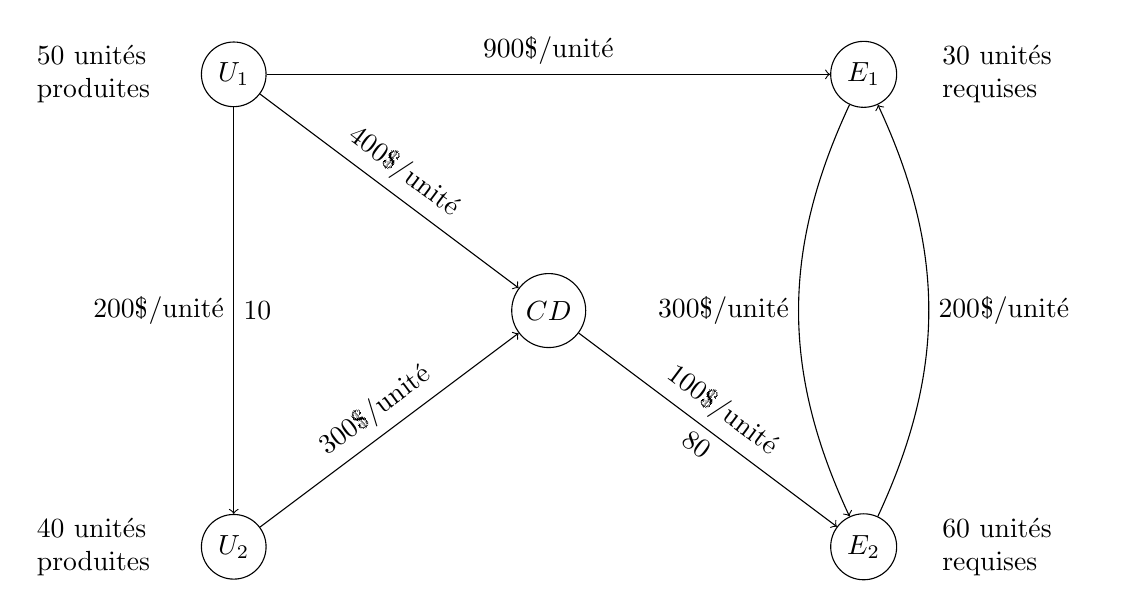
\begin{tikzpicture}[->]
\node [text width=2cm] at (-0.5,6) {50 unités produites};
\node[circle,draw] (U1) at (1,6) {$U_1$};
\node [text width=2cm] at (-0.5,0) {40 unités produites};
\node[circle,draw] (U2) at (1,0) {$U_2$};
\node [text width=2cm] at (11.0,6) {30 unités requises};
\node[circle,draw] (E1) at (9,6) {$E_1$};
\node [text width=2cm] at (11.0,0) {60 unités requises};
\node[circle,draw] (E2) at (9,0) {$E_2$};
\node[circle,draw](CD) at (5,3) {$CD$};
\path
  (U1) edge node [above,midway] {900\$/unité} (E1)
  (U1) edge node [left,midway] {200\$/unité} node[right,midway] {10} (U2)
  (U1) edge node [sloped,above,midway]{400\$/unité} (CD)
  (U2) edge node [sloped,above,midway] {300\$/unité} (CD)
  (CD) edge node [sloped,above,midway] {100\$/unité} node[sloped,below,midway] {80} (E2)
;
\draw [->] (E1) to [bend right=25] node [left,midway] {300\$/unité} (E2);
\draw [->] (E2) to [bend right=25] node [right,midway] {200\$/unité} (E1);
\end{tikzpicture}
\caption{Réseau de distribution}
\label{fig:network_linear}
\end{center}
\end{figure}

Comme d'ordinaire, pour formuler le modèle, identifions en premier lieu les variables d'intérêt. Nous désignerons par $x_{i,j}$ le nombre d'unités du produit transportées sur
l'arc $(i,j)$ (i.e. entre les sommets $i$ et $j$)
La fonction objectif (en chiifrant le montant total en centaines de dollars):
\[
\min z = 2 x_{U_1,U_2} + 4 x_{U_1,CD} + 9 x_{U_1,E_1} + 3 x_{U_2,CD} + x_{CD,E_2} + 3 x_{E_1,E_2} + 2 x_{E_2,E_1}.
\]
Les contraintes concernent tout d'abord la conservation du flot: en chaque sommet du réseau,
le flot sortant moins le flot entrant est égal au nombre d'unités produites dans le cas d'usine, l'opposé du nombre d'unités requises pour un entrepôt, et zéro pour le centre de distribution.
Nous devons en outre tenir compte de la capacité sur certains arcs.
Par exemple, pour l'arc $(U1,U2)$, nous avons
\[
x_{U_1,U_2} \leq 10.
\]
Il nous reste à préciser les traditionnelles contraintes de non-négativité:
\[
x_{i,j} \geq 0.
\]
Le modèle détaillé peut dès lors s'écrire de manière détaillée comme suit:
\begin{align*}
\min z & = 2 x_{U_1,U_2} + 4 x_{U_1,CD} + 9 x_{U_1,E_1} + 3 x_{U_2,CD} + x_{CD,E_2} + 3 x_{E_1,E_2} + 2 x_{E_2,E_1}. \\
\st & x_{U_1,U_2} + x_{U_1,CD} + x_{U_1,E_1} = 50, \\
& -x_{U_1,U_2} + x_{U_2,CD} = 40, \\
& -x_{U_1,CD} - x_{U_2,CD} + x_{CD,E_2} = -30, \\
& -x_{U_1,E_1} + x_{E_1,E_2} - x_{E_2,E_1} = -30, \\
& -x_{CD,E_2} - x_{E_1,E_2} + x_{E_2,E_1} = -60, \\
& x_{U_1,U_2} \leq 10, \\
& x_{CD,E_2} \leq 80, \\
& x_{U_1,U_2} \geq 0,\ x_{U_1,CD} \geq 0,\ x_{U_1,E_1} \geq 0,\ x_{U_2,CD} \geq 0,\ x_{CD,E_2} \geq 0,\ x_{E_1,E_2} \geq 0,\ x_{E_2,E_1} \geq 0.
\end{align*}
Il s'agit d'un problème de flot à coût minimum, que nous étudierons plus en détail au Chapitre~\ref{chap:networks}.
La solution optimale est
\[
(x^*_{U_1,U_2}, x^*_{U_1,CD}, x^*_{U_1,E_1}, x^*_{U_2,CD}, x^*_{CD,E_2}, x^*_{E_1,E_2}, x^*_{E_2,E_1}) = (0, 40, 10, 40, 80, 0, 20).
\]
Le nombre d'unités transportées doit toujours être une valeur entière, aussi l'hypothèse de continuité n'est pas satisfaite dans ce cas.
Néanmoins, dans ce cas particulier, la solution entière.
En fait, pour tout problème de flot à coût minimum (avec paramètres à valeurs entières), il existe toujours une solution optimale entière.
\end{example}

\section{La méthode du simplexe}

Dévloppée en 1947 par George Dantzig, la méthode du simplexe reste d'actualité pour résoudre des problèmes de grande taille.
Il s'agit d'une méthode algébrique basée sur la résolution de systèmes d'équations linéaires; nous nous intéressons ici uniquement aux systèmes d'équations linéaires avec un nombre $n$ de variables supérieur au nombre $m$ d'équations:
\[
Ax = b,
\]
où $x \in \RR^n$, $b \in \RR^m$ et $A \in \RR^{m \times n}$.
Dans ce cas, il y a trois possibilités:
\begin{enumerate}
\item
aucune solution;
\item
une et une seule solution;
\item
une infinité de solutions.
\end{enumerate}
Nous supposerons que toutes les variables sont positives.
Le second cas, avec une et seule solution, ne peut survenir que si $n = m$, et si la matrice $A$ est inversible, ce qui revient à exiger que nous avons éliminé au préalable toute équation pour s'écrire comme combinaison linéaire des autres équations.
Si nous n'avons qu'une seule solution admissible, elle est forcément optimale, par conséquent, nous ignorerons ce cas dans le reste du chapitre, et prendrons $n$ strictement supérieur à $m$.

Dans le cas où il y a une infinité de solutions, la méthode d'élimination de Gauss-Jordan permet d'identifier trois types de variables:
\begin{itemize}
\item
variables fixées;
\item
variables dépendantes;
\item
variables indépendantes.
\end{itemize}
\begin{example}[Préliminaires à l'algorithme du simplexe]
Considérons le système
\[
\begin{matrix}
x_1 & + & x_2 & + & x_3 & + & x_4 & = & 4, \\
x_1 & & & + & x_3 & + & x_4 & = & 3, \\
x_1 & + & x_2 & & & + & 2x_4 & = & 2.
\end{matrix}
\]
Nous pouvons le réécrire sous la forme
\[
\begin{matrix}
x_1 & + & & & & + & 2x_4 & = & 1, \\
& & x_2 & & & & & = & 1, \\
& & & & x_3 & - & x_4 & = & 2.
\end{matrix}
\]
La variable $x_2$ est fixée, comme elle ne peut prendre que la valeur 1, sans considération pour les autres variables. A l'opposée, $x_4$ est indépendante, comme elle peut prendre n'importe quelle valeur dans $\RR$. $x_1$ et $x_3$ sont quant à elles dépendantes: le choix de $x_4$ fixe leur valeur, et de plus, il n'est pas possible de les éliminer en combinant des équations entre elles (au contraire de $x_4$).
\end{example}

\subsection{Solution de base}

Il s'agit de la solution obtenue en fixant toutes les variables indépendantes à zéro.
Nous qualifierons de {\sl variables hors-base} les variables indépendantes fixées à zéro.
Les autres variables seront dites {\sl variables de base}.
Une solution de base est {\sl réalisable} (ou {\sl admissible}) lorsque toutes les variables de base ont une valeur positive.
Une solution de base réalisable est {\sl dégénérée} lorsqu'au moins une variable de base a la valeur 0.
Il est possible de montrer qu'une solution de base réalisable est un sommet du polyèdre.

\begin{example}[Préliminaires à l'algorithme du simplexe: solution de base]
Dans l'exemple, la solution de base est
\[
x_1 = 1,\ x_2 = 1,\ x_3 = 2.
\]
Elle est réalisable et non dégénérée.
\end{example}

\subsubsection{Pivot}

Il est facile de changer le statut des variables par des opératins élémentaires.
\begin{example}[Préliminaires à l'algorithme du simplexe: pivot]
\[
\begin{matrix}
x_1 & + & & & & + & 2x_4 & = & 1, \\
& & x_2 & & & & & = & 1, \\
& & & & x_3 & - & x_4 & = & 2.
\end{matrix}
\]
peut se réécrire comme
\[
\begin{matrix}
x_1 & & & + & 2x_3& & & = & 5, \\
& & x_2 & & & & & = & 1, \\
& & & & -x_3 & + & x_4 & = & -2.
\end{matrix}
\]
Dans cette nouvelle solution de base, nous avons
\begin{itemize}
\item
variable hors-base: $x_3$;
\item
variables de base: $x_1$, $x_2$, $x_4$;
\item
solution de base non réalisable: $x_1 = 5$, $x_2 = 1$, $x_4 = -2$.
\end{itemize}
\end{example}
Le {\sl pivot} est une opération consistant à remplacer une variable de base par une variable hors base pour obtenir une nouvelle solution de base, dite {\sl adjacente}.

\begin{example}[Wyndor Glass]
Rappelons que pour cet exemple, les contraintes fonctionnelles sont
\begin{eqnarray*}
x_1 & \leq 4 \\
2x_2 & \leq 12 \\
3x_1 + 2x_2 & \leq 18
\end{eqnarray*}
Au lieu d'inégalités, nous voudrions des égalités.
Pour ce faire, nous ajoutons des variables d'écart (en anglais ``slack variables'') supérieures à 0:
\[
\begin{matrix}
x_1 & & + x_3 & & & = 4 \\
& 2x_2 & & + x_4 & &  = 12\\
3x_1 & + 2x_2 & & & +x_5 & = 18
\end{matrix}
\]
Les variables hors-base sont $x_1$ et $x_2$. Fixons-les à 0.
Nous obtenons comme solution de base
\[
(x_1, x_2, x_3, x_4, x_5) = (0, 0, 4, 12, 18).
\]
Effectuons un pivot, en remplaçant la variable hors-base par une des variables de base actuelles.
Reste à déterminer comment la choisir.
Nous souhaitons en premier lieu que la nouvelle solution de base soit réalisable.
Dans cette solution de base, on aura toujours $x_1 = 0$, et une des variables d'écart deviendra une variable hors-base, donc prendre la valeur 0.
En exploitant le système linéaire précédent et la positivité des variables, nous avons
\[
\begin{matrix}
x_1 & = & 4 & -x_3 & & \geq 0 & & 4 & & \geq x_3 \\
x_4 & = & 12 & & -2x_2 & \geq 0 & \Leftrightarrow & 12 & -2x_2 & \geq 0 \\
x_5 & = & 18 & -3x_1 & -2x_2 & \geq 0 & & 18 & -2x_2 & \geq 0
\end{matrix}
\]
En exploitant les inégalités
\begin{align*}
x_4 &= 12 - 2x_2 \geq 0 \\
x_5 &= 18 - 2x_2 \geq 0,
\end{align*}
nous obtenons
\begin{align*}
x_2 &\leq 12/2 = 6 \\
x_2 &\leq 18/2 = 9.
\end{align*}
Par conséquent, en posant $x_2 = 6$, nous obtenons $x_4 = 0$, alors que si nous augmentons d'avantage $x_2$, la solution devient non réalisable.
Nous effectuons comme pivot le remplacement de la variable de base $x_4$ (qui deviendra hors-base) par $x_2$.
Nous obtenons alors le système suivant:
\[
\begin{matrix}
x_1 & & + x_3 & & & = 4 \\
& x_2 & & + \frac{1}{2} x_4 & &  = 6\\
3x_1 & & & -x_4 & +x_5 & = 6,
\end{matrix}
\]
qui donne la solution de base:
\[
(x_1, x_2, x_3, x_4, x_5) = (0,6,4,0,6).
\]
Nous effectuons ensuite un pivot pour que la variable $x_1$ {\sl entre dans la base} (i.e. devienne une variable de base).
Comme $x_4 = 0$,
\[
\begin{matrix}
x_3 & = & 4 & -x_1 & & \geq 0 \\
x_5 & = & 6 & & -3x_1 & \geq 0
\end{matrix}
\ 
\Leftrightarrow
\ 
\begin{matrix}
x_1 & \leq & 4 \\
x_1 & \leq & 2
\end{matrix}
\]
En posant $x_1 = 2$, nous obtenons $x_5 = 0$.
Le pivot revient à remplacer la variable de base $x_5$ par $x_1$.
Le système obtenu est alors :
\[
\begin{matrix}
& & x_3 & + \frac{1}{3} x_4 & -\frac{1}{3} x_5 & = 2 \\
& x_2 & & +\frac{1}{2}x_4 & & = 6 \\
x_1 & & & -\frac{1}{3}x_4 & +\frac{1}{3}x_5 & = 2
\end{matrix}
\]
La solution de base correspondante est
\[
(x_1, x_2, x_3, x_4, x_5) = (2,6,2,0,0).
\]
\begin{figure}[htbp]
\begin{center}
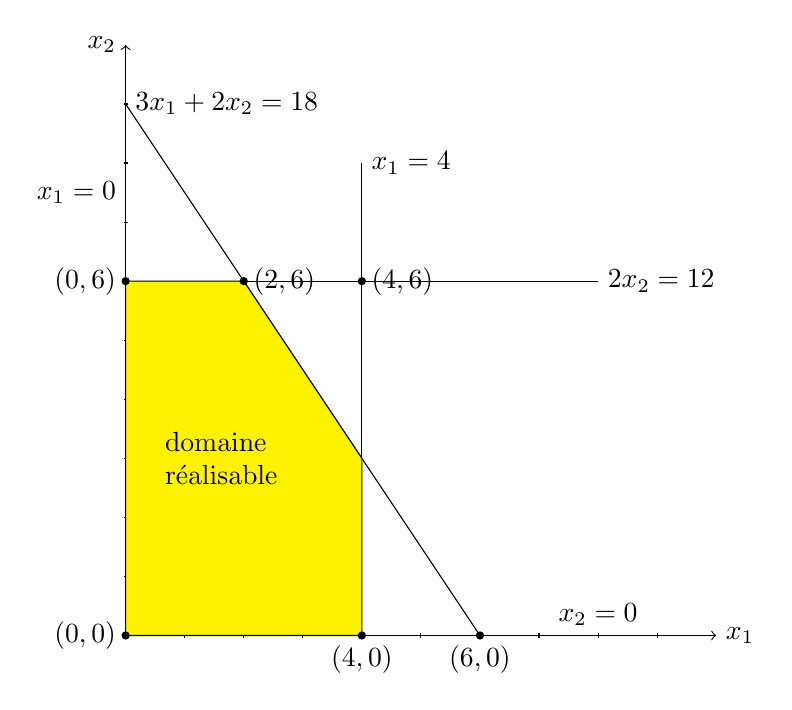
\begin{tikzpicture}[scale=0.75]
\draw[->] (0,0) -- (10,0) node[below,right] {$x_1$};
\draw[->] (0,0) -- (0,10) node[above,left] {$x_2$};
\draw (6,0) -- (0,9) node[above,right] {$3x_1 + 2x_2 = 18$};
\draw (0,6) -- (8,6) node[right] {$2x_2 = 12$};
\draw (4,0) -- (4,8) node[above,right] {$x_1 = 4$};
\node [left] at (0,7.5) {$x_1 = 0$};
\node [above] at (8.0,0) {$x_2 = 0$};

\foreach \x in {0,1,2,3,4,5,6,7,8,9}
  \draw (\x,1pt) -- (\x,-1pt) node[anchor=north] {};
\foreach \y in {0,1,2,3,4,5,6,7,8,9}
  \draw (1pt,\y) -- (-1pt,\y) node[anchor=east] {};

\filldraw[fill=yellow]
  (0,0) -- (0,6) -- (2,6) -- (4,3) -- (4,0) -- (0,0);
 
\draw (0,0) node[left] {$(0,0)$};
\fill (0,0) circle (2 pt);
\draw (0,6) node[left] {$(0,6)$};
\fill (0,6) circle (2 pt);
\draw (2,6) node[above,right] {$(2,6)$};
\fill (2,6) circle (2 pt);
\draw (4,6) node[above,right] {$(4,6)$};
\fill (4,6) circle (2 pt);
\draw (4,0) node[below] {$(4,0)$};
\fill (4,0) circle (2 pt);
\draw (6,0) node[below] {$(6,0)$};
\fill (6,0) circle (2 pt);

 \draw (2,3) node[text width=2cm,text ragged] {domaine réalisable};

\end{tikzpicture}
\end{center}
\caption{exemple Wyndor Glass}
\label{fig:wyndor_simplex}
\end{figure}
\end{example}

\subsection{Interprétations}

\subsubsection{Interprétation géométrique}

Une solution de base réalisable correspond à un point extrême du domaine réalisable.
Un pivot correspond à un déplacement d'un point extrême à un autre qui lui est {\sl adjacente}, i.e. toutes les variables hors-base sauf une sont les mêmes.
La méthode du simplexe peut se résumer comme suit.
\begin{enumerate}
\item
Nous débutons avec une solution de base réalisable initiale (un
{\sl point extrême}).
\item
A chaque itération, nous effectuons un pivot, passant ainsi à une
solution de base réalisable adjacente (un point extrême adjacent).
\item
L'algorithme s'arrête lorsqu'il identifie une solution de base réalisable
optimale (un point extrême correspondant à une solution optimale).
\end{enumerate}

\subsubsection{Interprétation des variables d'écart}

\begin{example}
Dans la solution optimale du problème Wyndor Glass, nous avons x3 = 2, x4 = x5 = 0.
Cela indique que les deux dernières ressources (temps aux usines 2 et 3) sont pleinement utilisées.
Une partie de la première ressource (temps à l'usine 1) n'est pas utilisée: 2 heures
\end{example}

\subsection{Critère d'optimalité}

\begin{example}[Wyndor Glass: critère d'optimalité]
Exprimons l'objectif en fonction des variables hors-base dans la solution optimale
Rappelons que dans cette solution, nous avons
\[
\begin{matrix}
& x_2 & & +\frac{1}{2}x_4 & & = 6 \\
x_1 & & & -\frac{1}{3}x_4 & +\frac{1}{3}x_5 & = 2
\end{matrix}
\]
Après substitution dans l'objectif, nous obtenons
\begin{align*}
\max z\ & = 3 x_1 + 5 x_2 \\
& = 3 \left(2 + \frac{1}{3} x_4 - \frac{1}{3} x_5 \right) + 5 \left(6 - \frac{1}{2} x_4 \right) \\
& = 36 - \frac{3}{2} x_4 - x_5.
\end{align*}
Toute solution réalisable $(x_1, x_2, x_3, x_4, x_5)$ satisfait
\[
z = 36 + 0 x_1 + 0 x_2 + 0 x_3 - \frac{3}{2} x_4 - x_5 \leq 36.
\]
\end{example}

Le critère d'optimalité s'énonce ainsi comme suit:
étant donné que l'objectif s'exprime uniquement en fonction des variables hors-base de la solution de base réalisable courante, si les coefficients de ces variables dans l'objectif sont tous négatifs ou nuls, alors la solution de base réalisable courante est optimale.
Les coefficients des variables hors-base dans l'objectif sont appelés {\sl coûts réduits} (ou coûts relatifs).

Si au moins un coût réduit est positif pour la solution de base courante, nous n'avons pas encore atteint une solution optimale.
Il faut par conséquent effectuer au moins un pivot, mais quelle variable doit-on faire entrer dans la base.
Regardons celle dont le coût réduit est le plus grand parmis toutes les variables hors-base, vu que cette variable fournit la plus grande augmentation marginale (par unité) de la valeur de l'objectif. Ce qui ne signifie toutefois pas la plus grande augmentation globale!

Vu que nous faisons entrer une variable dans la base, nous devons également choisir la variable qui va sortir de la base en tentant de garder toutes les variables non négatives.
Supposons que $x_j$ est la variable d'entrée. Chaque variable de base $x_i$ s'exprime alors en fonction de la variable d'entrée (puisque les autres variables hors-base sont nulles):
\[
x_i = \overline{b}_i - \overline{a}_{ij}x_j.
\]
Dans cette expression, les coefficients $\overline{b}_i$ et $\overline{a}_{ij}$ sont obtenus suite à plusieurs pivots.
Mais nous avons nécessairement $\overline{b}_i$ positif (en partant d'un $b$ positif).
%En effet, les $b_i$ initiaux doivent être positifs, sinon la solution triviale nulle n'est pas réalisable. Les opérations de pivot maintiennent la positivité. %POURQUOI???
Pour que toutes les variables demeurent non négatives suite au pivot, nous devons avoir
\[
x_i = \overline{b}_i - \overline{a}_{ij}x_j \geq 0,
\]
soit, en d'autres termes,
\[
\overline{a}_{ij}x_j \leq \overline{b}_i.
\]

Si $\overline{a}_{ij}$ est négatif, cette inégalité ne limite pas l'augmentation de $x_j$.
Si cette condition est satisfaite pour tous les $i$, nous pouvons donc augmenter indéfiniment $x_j$; l'objectif est non borné.
Si $\overline{a}_{ij}$ est strictement positif, l'inégalité limite l'augmentation de $x_j$.
Nous prendrons comme variable de sortie celle qui atteint
\[
\min \left\lbrace \left. \frac{\overline{b}_i}{\overline{a}_{ij}} \right| \overline{a}_{ij} > 0\right\rbrace.
\]

\begin{algo}{Simplexe}
\begin{enumerate}
\item
Obtenir une solution de base réalisable.
\item
Vérifier le critère d'optimalité: si les coûts réduits de toutes les variables hors-base sont négatifs ou nuls, stop.
\item
Choisir la variable $x_j$, soit celle qui a le coût réduit le plus élevé.
\item
Déterminer la variable de sortie:
\[
\min \left\lbrace \left. \frac{\overline{b}_i}{\overline{a}_{ij}} \right| \overline{a}_{ij} > 0\right\rbrace.
\]
\item
Effectuer un pivot et déterminer une nouvelle solution de base réalisable. Retour à l'étape 2.
\end{enumerate}
\end{algo}

\begin{example}[Production]
Une entreprise fabrique quatre produits.
La fabrication de chaque produit nécessite une certaine quantité de ressources.
Les ressources consommées, les stocks des ressources et les bénéfices des
produits sont récapitulés dans la Table~\ref{tab:prod_simplexe}.
\begin{table}[htbp]
\begin{center}
\begin{tabular}{|c|cccc|c|}
\hline
Produit & 1 & 2 & 3 & 4 & Stock \\
\hline
Ressource A & 2 & 4 & 5 & 7 & 42 \\
Ressource B & 1 & 1 & 2 & 2 & 17 \\
Ressource C & 1 & 2 & 3 & 3 & 24 \\
\hline
Profit & 7 & 9 & 18 & 17 & - \\
\hline
\end{tabular}
\end{center}
\caption{Données de production}
\label{tab:prod_simplexe}
\end{table}
Nous souhaitons établir un plan de production de façon à maximiser le chiffre d'affaires.

Soient $x_1$, $x_2$, $x_3$ et $x_4$ les quantités respectives de produits 1, 2, 3, 4.
Nous avons le problème de programmation linéaire sous forme standard
\begin{align*}
\max z &= 7x_1 + 9x_2 + 18x_3 + 17x_4 \\
\st & 2x_1 + 4x_2 + 5x_3 + 7x_4 \leq 42 \\
& x_1 + x_2 + 2x_3 + 2x_4 \leq 17 \\
& x_1 + 2x_2 + 3x_3 + 3x_4 \leq 24 \\
& x_1,\ x_2, x_3, x_4 \geq 0.
\end{align*}
Introduisons trois variables d'écart $x_5$, $x_6$, $x_7$, qui mesurent pour chaque ressource l'écart entre la quantité initialement disponible et la quantité consommée par le plan de fabrication donné par les variables de décision $x_1$, $x_2$, $x_3$, $x_4$:
\begin{align*}
\max z &= 7x_1 + 9x_2 + 18x_3 + 17x_4 \\
\st & 2x_1 + 4x_2 + 5x_3 + 7x_4 + x_5 = 42 \\
& x_1 + x_2 + 2x_3 + 2x_4 + x_6 = 17 \\
& x_1 + 2x_2 + 3x_3 + 3x_4 + x_7 = 24 \\
& x_1,\ x_2, x_3, x4 \geq 0.
\end{align*}
Cette formulation permet d'exprimer facilement les variables d'écart comme fonctions affines des variables de décision:
\begin{align*}
x_5 &= 42 - 2x_1 - 4x_2 - 5x_3 - 7x_4 \\
x_6 &= 17 - x_1 - x_2 - 2x_3 - 2x_4 \\
x_7 &= 24 - x_1 - 2x_2 - 3x_3 - 3x_4 \\
z &= 7x_1 + 9x_2 + 18x_3 + 17x_4
\end{align*}
Le tableau ci-dessus est appelé un {\sl dictionnaire}.
Les variables $x_5$, $x_6$, $x_7$ sont les variables de base et $x_1$, $x_2$, $x_3$, $x_4$ sont des variables hors-base.
La solution de base associée au dictionnaire est obtenue en donnant la valeur 0 à toutes les variables hors-base.
La solution basique correspondant au dictionnaire ci-dessus est donc
\[
(x_1, x_2, x_3, x_4, x_5, x_6, x_7) = (0, 0, 0, 0, 42, 17, 24).
\]
Le bénéfice correspondant est $z = 0$;
on ne produit rien, on ne consomme aucune ressource et on ne gagne rien.
Néanmoins, c'est une solution réalisable, car elle satisfait toutes les contraintes.

En partant de cette solution basique, nous cherchons à améliorer le bénéfice.
Nous sélectionnons la variable hors-base de coût réduit maximum, i.e. $x_3$, et gardons les autres variables hors-base à zéro.
Il est évident que si on fait croître $x_3$ à partir de 0, les autres variables hors-base restant nulles, la valeur de la fonction $z$ croît.
Nous cherchons à augmenter au plus la fonction objectif tout en gardant la solution reste réalisable.
Les contraintes sur l'augmentation de $x_3$ sont:
\begin{align*}
x_5 \geq 0 \Rightarrow 42 - 5x_3 \geq 0 \Rightarrow x_3 \leq 8.4 \\
x_6 \geq 0 \Rightarrow 17 - 3x_3 \geq 0 \Rightarrow x_3 \leq 8.5 \\
x_7 \geq 0 \Rightarrow 24 - 3x_3 \geq 0 \Rightarrow x_3 \leq 8.
\end{align*}
La plus restrictive de ces contraintes est $x_3 \leq 8$.
L'interprétation géométrique est la suivante: en partant du sommet $(0, 0, 0, 0)$ du polyèdre des contraintes, nous nous déplaçons sur une arête de ce polyèdre.
Le premier hyperplan rencontré est $x_7 = 0$.
Nous arrivons alors dans un nouveau sommet, à l'intersection des hyperplans $x_1 = 0$, $x_2 = 0$, $x_4 = 0$, $x_7 = 0$.

Nous allons faire un changement de dictionnaire, i.e. un pivot, en échangeant les rôles de $x_3$ et $x_7$.
Nous utilisons la troisième équation du premier dictionnaire pour exprimer $x_3$ en fonction de $x_1$, $x_2$, $x_4$ et $x_7$:
\[
x_3 = 8 - \frac{1}{3} x_1 - \frac{2}{3} x_2 - x_4 - \frac{1}{3} x_7.
\]
Nous remplaçons ensuite $x_3$ par cette expression dans les autres équations du dictionnaire:
\begin{align*}
x_5 &= 2 - \frac{1}{3}x_1 - \frac{2}{3}x_2 + \frac{5}{3}x_7 - 2x_4 \\
x_6 &= 1 - \frac{1}{3}x_1 + \frac{1}{3}x_2 + \frac{2}{3}x_7 \\
x_3 &= 8 - \frac{1}{3}x_1 - \frac{2}{3}x_2 - \frac{1}{3}x_7 - x_4 \\
z &= 144 + x_1 - 3x_2 - 6x_7 - x4.
\end{align*}
La variable $x_7$ est sortie de la base et la variable $x_7$ est entrée dans la base.
La nouvelle base est par conséquent $x_5$, $x_6$, $x_3$.
La solution basique associée au nouveau dictionnaire est $x_1 = x_2 = x_7 = x_4 = 0$, $x_5 = 2$, $x_6 = 1$, $x_3 = 8$.
Elle correspond au sommet de coordonnées $(0, 0, 8, 0)$ du polyèdre de contraintes.
Cette solution définit un plan de production beaucoup plus intéressant: nous fabriquons 8 unités du produit 3 ($x_3 = 8$) en consommant entièrement la ressource C ($x_7 = 0$).
Il nous reste $x_5 = 2$ unités de la ressource A et $x_6 = 1$ unité de B.
Le bénéfice est $z = 144$.

Dans la nouvelle expression de la fonction $z$, nous voyons que seule la variable $x_1$ a un coefficient positif.
Nous décidons de faire entrer $x_1$ en base, et ainsi de parcourir une nouvelle arête du polyèdre des contraintes.
Nous avons les limites suivantes sur l'augmentation de $x_1$:
\begin{align*}
x_5 \geq 0 \Rightarrow x_1 \leq 6
x_6 \geq 0 \Rightarrow x_1 \leq 3
x_3 \geq 0 \Rightarrow x_1 \leq 24
\end{align*}
d'où $x_1 \leq 3$
Nous faisons sortir $x_6$ de la base faisons entrer $x_1$ à sa place.
Nous obtenons le dictionnaire suivant:
\begin{align*}
x_5 &= 1 + x_6 - x_2 + x_7 - 2x_4 \\
x_1 &= 3 - 3x_6 + x_2 + 2x_7 \\
x_3 &= 7 + x_6 - x2 - x_7 - x_4 \\
z &= 147 - 3x_6 - 2x_2 - 4x_7 - x_4.
\end{align*}
La solution de base associée est $x_6 = x_2 = x_7 = x_4 = 0$, $x_5 = 1$, $x_1 = 3$, $x_3 = 7$, correspond au sommet $(3, 0, 7, 0)$ du polyèdre des contraintes.
Elle définit le plan de production suivant: nous fabriquons 3 unités du produit 1 et 7 unités du produit 3.
Il ne nous reste qu'une unité de la ressource A.
Le bénéfice est $z = 147$.
De plus, tous les coûts réduits sont négatifs, aussi la solution est optimale.
\end{example}

\subsection{Adaptation à d'autres formes de modèles}

Tout modèle de programmation linéaire peut se ramener à la forme suivante:
\begin{align*}
\max \ & \sum_{j = 1}^n c_j x_j \\
\st & \sum_{j = 1}^n a_{ij} x_j + x_{n+i} = b_i,\ i = 1,2,\ldots,m\\
& x_j \geq 0,\ j = 1,2,\ldots,n, \\
& x_{n+i} \geq 0,\ i = 1,2,\ldots,m.
\end{align*}
Nous supposons de plus que $b_i$ est positif, $i = 1,2,\ldots,m$.
Sous cette forme, il est facile d'initialiser la méthode du simplexe en ajoutant des variables d'écart, et en les prenant comme variables de base.
Cela revient de plus à considérer l'origine comme solution initiale, et il est facile d'effectuer les opérations de pivot.
Le situation se complique avec d'autres formes fonctionnelles pour les contraintes, en particulier dans la recherche d'une solution de base initiale.

\subsubsection{Transformation du $\min$ au $\max$}

Supposons que nous devions minimiser l'objectif au lieu de le maximiser.
Nous utilisons la propriété
\[
\min \sum_{j=1}^n c_j x_j = -\max -\sum_{j=1}^n c_j x_j.
\]
Nous résolvons le problème de maximisation en changeant les signes des coefficients dans l'objectif.
La valeur optimale du problème de minimisation est l'opposé de celle du problème de maximisation.

\subsubsection{Transformation des inégalités en égalités}

Si $\sum_{j=1}^n a_{ij} x_j \leq b_i$, il y a deux cas:
\begin{enumerate}
\item
$b_i \geq 0$: nous ajoutons une variable d'écart positive $x_{n_i}$:
\[
\sum_{j = 1}^n a_{ij} x_j + x_{n+i} = b_i.
\]
\item
$b_i < 0$: nous multiplions l'inégalité par -1, pour se ramener au cas développé ci-dessous.
\end{enumerate}

Si $\sum_{j=1}^n a_{ij} x_j \geq b_i$, nous avons à nouveau deux cas possibles:
\begin{enumerate}
\item
$b_i \leq 0$: nous multiplions l'inégalité par -1, pour se ramener au cas développé précédemment.
\item
$b_i > 0$: nous soustrayons une variable de surplus positive $x_{0i}$:
\[
\sum_{j = 1}^n a_{ij} x_j - x_{0i} = b_i.
\]
Nous nous ramenons alors au cas d'ajout de variables artificielles.
\end{enumerate}

\subsection{Obtention d'une base admissible initiale}

\subsubsection{Ajout de variables artificielles}

Si $\sum_{j = 1,\ldots,n} a_{ij}x_j = b_i$ et qu'aucune variable n'est isolée (une variable est isolée si elle à coefficient 1 dans cette équation et à coefficient 0 dans les autres):
\begin{enumerate}
\item
nous ajoutons une variable artificielle $x_{n+1} \geq 0$, dont l'unique but est de fournir une variable de base initiale pour cette contrainte;
\item
nous lui associons un profil très négatif: $-M$
\begin{align*}
\max\ & \sum_{j = 1,\ldots,n} c_{j}x_j - M x_{n+i} \\
\st & \ldots \\
& \sum_{j = 1,\ldots,n} a_{ij}x_j + x_{n+i} = b_i \\
& \ldots
\end{align*}
\end{enumerate}
Le seul but des variables artificielles est de pouvoir initialiser l'algorithme du simplexe en produisant une solution de base réalisable initiale.
Si le problème est réalisable, nous devrions avoir $x_{n+i} = 0$.
Deux méthodes peuvent être considérées.
\begin{enumerate}
\item
La {\sl méthode du grand $M$} consiste à optimiser en utilisant une fonction objective formée de la fonction de coût initiale et de la somme, très fortement pénalisée, des variables artificielles.
\item
La {\sl méthode à deux phases} se déroule comme suit:
\begin{description}
\item[Phase 1]
Trouver une solution réalisable en minimisant la somme des variables artificielles.
\item[Phase 2]
Optimiser en revenant à la fonction de coût initial à partir de la solution initiale trouvée dans la phase 1.
\end{description}
\end{enumerate}

\begin{example}
Considérons le programme
\begin{align*}
\min z & = 0.4 x_1 + 0.5 x_2 \\
\st & 0.3 x_1 + 0.1 x_2 \leq 2.7 \\
& 0.5 x_1 + 0.5 x_2 = 6 \\
& 0.6 x_1 + 0.4 x_2 \geq 6 \\
& x_1 \geq 0,\ x_2 \geq 0.
\end{align*}
Nous devons tout d'abord transformer le système de contraintes afin de pouvoir traiter un système linéaire:
\begin{align*}
0.3 x_1 + 0.1 x_2 + x_{s1} & = 2.7 \\
0.5 x_1 + 0.5 x_2 & = 6 \\
0.6 x_1 + 0.4 x_2 - x_{s2} & = 6 \\
x_{s1} \geq 0,\ x_{s2} \geq 0. &
\end{align*}
En ajoutant les variables artificielles, nous obtenons
\begin{align*}
0.3 x_1 + 0.1 x_2 + x_{s1} & = 2.7 \\
0.5 x_1 + 0.5 x_2 + x_{a2} & = 6 \\
0.6 x_1 + 0.4 x_2 - x_{s2} +x_{a3} & = 6 \\
x_{s1} \geq 0,\ x_{s2} \geq 0,\ x_{a2} \geq 0,\ x_{a3} & \geq 0. %
\end{align*}
Afin de démarrer la méthode du simplexe, nous appliquons une des deux méthodes précédentes.
Méthode à deux phases:
\begin{description}
\item[Phase 1] minimiser $x_{a2} + x_{a3}$ jusqu'à obtenir une valeur optimale nulle (si le programme linéaire à une solution réalisable).
\item[Phase 2] minimiser $0.4 x_1 + 0.5 x_2$.
\end{description}
Méthode du grand $M$:
\[
\min 0.4 x_1 + 0.5 x_2 + Mx_{a2} + Mx_{a3}
\]
\end{example}

\subsection{Variables à valeurs quelconques}

Si une variable $x_j$ peut prendre des valeurs négatives, nous introduisons deux variables $x_j^+ \geq 0$ et $x_j^- \geq 0$.
Nous posons alors
\[
x_j = x_j^+ - x_j^-.
\]
Une autre possible, si $x_j \geq L_j$, où $L_j$ est une constante négative, consiste à poser
\[
x_j^+ = x_j - L_j \geq 0.
\]

\section{Dualité}

\subsection{Motivation}

\begin{example}[Wyndor Glass: dualité]
Supposons qu'une compagnie partenaire de Wyndor Glass, appelée Dual Glass, aimerait louer du temps aux usines afin de fabriquer des lots de produits.
Quel prix horaire pour chaque usine devrait-elle demander de telle sorte que le résultat soit équitable, soit aucun profit ni perte pour aucun des deux partenaires?

Dénotons les nouvelles variables de décision par $y_i$, le prix de location horaire à l'usine $i$, et reprenons les données du problèmes telles qu'exprimé précédemment dans la Table~\ref{tab:wyndor}.
\begin{center}
\begin{tabular}{|c|c|c|c|}
\hline
& Produit 1 & Produit 2 & Capacité de \\
& Temps de prod. (h) & Temps de prod. (h)& production (h)\\
\hline
Usine 1 & 1 & 0 & 4 \\
\hline
Usine 2 & 0 & 2 & 12 \\
\hline
Usine 3 & 3 & 2 & 18 \\
\hline
\end{tabular}
\end{center}
Dual Glass cherche a minimiser le prix total qu'elle devra payer pour le temps loué aux trois usines.
Le prix total pour chaque usine peut etre exprimé comme 
\[
\mbox{temps de production maximum (h)} \times \mbox{prix}
\]
pour louer du temps (\$/h).
L'objectif est par conséquent
\[
\min w = 4 y_1 + 12 y_2 + 18 y_3.
\]
Les contraintes assurent que le prix total associé à la fabrication d'un lot de chaque produit ne doit pas être inférieure au profit (\$/lot) qu'en retire Wyndor Glass.
Le prix total associé à un produit peut être exprimé comme le temps consacré à la production de chaque lot (h/lot) multiplié par le prix pour louer du temps (\$/h).
La contrainte associée au produit 1 peut s'exprimer comme
\[
y_1 + 3 y_3 \geq 3.
\]
La contrainte associée au produit 2 est
\[
2y_2 + 2 y_3 \geq 5.
\]
Nous obtenons ainsi le modèle pour Dual Glass, appelé {\sl modèle dual}:
\begin{align*}
\min w\ &= 4y_1 + 12y_2 + 18y_3 \\
\st & y_1 + 3y_3 \geq 3 \\
& 2y_2 + 2y_3 \geq 5 \\
& y_1,\ y_2,\ y_3 \geq 0.
\end{align*}
Pour rappel, le modèle pour Wyndor Glass, dit modèle primal est
\begin{align*}
\max z\ &= 3x_1 + 5x_2 \\
\st & x_1 \leq 4 \\
& 2x_2 \leq 12 \\
& 3x_1 + 2x_2 \leq 18
\end{align*}

Rappelons que pour la solution de base optimale du problème Wyndor Glass, l'objectif s'écrit:
\[
z = 36 - \frac{3}{2}x_4 - x_5.
\]
$x_4$ et $x_5$ sont les variables hors base et les coefficients $-\frac{3}{2}$ et $-1$ sont leurs {\sl coûts réduits}.
Si on augmente la valeur de $x_4$ de une unité, le profit diminue de $\frac{3}{2}$.
$x_4$ est également la variable d'écart associée à la contrainte de ressource pour l'usine 2:
\[
2x_2+x_4 = 12.
\]
Augmenter $x_4$ d'une unité signifie par conséquent diminuer le terme de droite correspondant de 1.
En effet, si Wyndor Glass loue a Dual Glass une heure de temps de production à l'usine 2:
\begin{itemize}
\item
la capacité à l'usine 2 diminue de 1 heure (diminution d'une unité du terme de droite);
\item
la valeur de l'objectif diminue de $\frac{3}{2}$.
\end{itemize}
Pour retrouver un profit total égal, il faudra donc demander un prix de $\frac{3}{2}$ (1500\$) pour chaque heure de temps louée à l'usine 2.
De manière générale, la solution optimale du dual est donnée par l'opposé des coûts réduits des variables d'écart (aussi appelés {\sl multiplicateurs optimaux}, ou {\sl shadow prices} en anglais).
Dans notre exemple:
\[
  y_1 = 0,\ y_2 = \frac{3}{2},\ y_3 = 1.
\]
Le prix de la variable $y_1$ est fixé à 0:
\begin{itemize}
\item
Wyndor Glass n'exige rien pour une heure louée à l'usine 1, ce qui se justifie par le fait qu'il lui reste du temps de production non utilisé (la variable d'écart $x_3$ est strictement positive).
\item
Un prix strictement positif ferait augmenter le profit, et la solution ne serait plus équitable.
\end{itemize}
Les prix des autres variables est strictement positif:
\begin{itemize}
\item
puisque le temps de production est utilisé pleinement, louer une heure à Dual Glass revient à perdre une heure de production, donc à réduire le profit total;
\item
pour retrouver le même profit, il faut exiger un prix égal au multiplicateur optimal, égal à l'opposé du coût réduit.
\end{itemize}
Nous pouvons constater des écarts complémentaires: pour tout $i$, nous avons
\[
  x_{n+i}.y_i = 0.
\]
\end{example}

Tout modèle de programmation linéaire possède un dual.
A tout programme linéaire sous forme standard
\begin{align*}
\max z &= c^Tx\\
\st & Ax \leq b, \\
& x \geq 0,
\end{align*}
nous associons le programme dual
\begin{align*}
\min w &= b^Ty\\
\st & A^Ty \geq c, \\
& y \geq 0,
\end{align*}
Nous obtenons ainsi un couple primal-dual, avec les relations suivantes entre les deux
modèles.
\begin{center}
\begin{tabular}{|c|c|}
\hline
{\bf Primal} & {\bf Dual} \\
\hline
Variable & Contrainte \\
\hline
Contrainte & Variable \\
\hline
$\max$ & $\min$ \\
\hline
Profit unitaire & Terme de droite \\
\hline
Terme de droite & Coût unitaire \\
\hline
Ligne & Colonne \\
\hline
Colonne & Ligne \\
\hline
Contrainte $\leq$ & Contrainte $\geq$ \\
\hline
\end{tabular}
\end{center}
Si un modele de programmation linéaire possède une solution optimale, il
en est de même pour son dual, et les valeurs optimales des deux modèles sont égales.

La solution optimale du dual correspond aux multiplicateurs optimaux.
Nous pouvons les lire directement dans le tableau optimal du simplexe: ce sont les coefficients dans la ligne correspondant à l'objectif.
Le coût réduit (correspondant à l'opposé du coefficient dans la ligne de l'objectif)
mesure la variation de l'objectif entraîné par une augmentation d'une unité de la valeur de la variable hors-base associée.

\subsection{Analyse de sensibilité}

% paragraphe à retravailler
En général, le coût réduit d'une variable hors-base indique le changement dans l'objectif apporté par une augmentation d'une unité de la valeur de cette variable.
Pour les variables d'écart, ce principe peut se formuler ainsi: le coût réduit d'une variable d'écart hors-base indique le changement dans l'objectif apporté par une diminution d'une unité du terme de droite associé.
Ceci est un exemple d'analyse de sensibilité: un paramètre (ici, un terme de droite) est modifié et nous mesurons la sensibilité de la solution optimale à ce changement.

Nous pouvons aussi mesurer la sensibilité de la solution optimale à un changement d'un terme de droite ou d'un coefficient dans l'objectif en resolvant à nouveau le modèle modifié.

\begin{example}[Wyndor Glass: sensibilité]
Une analyse de sensibilité complète nous apprendrait ce qui suit.
\begin{itemize}
\item
Les multiplicateurs optimaux (Shadow Prices) sont 0, 1500
et 1000.
\item
La capacité à l'usine 3 peut prendre n'importe quelle valeur entre 12h et 24h sans changer la solution optimale du dual.
\item
Le profit unitaire pour le produit 1 peut prendre n'importe quelle valeur entre 0 et 7500\$ sans changer la solution optimale du primal.
\end{itemize}
\end{example}

\begin{example}
Considérons un fermier cultivant trois types de plantes (maïs, blé, coton), en utilisant des ressources de terre et de main d'oeuvre.
Les revenus nets venant de la culture du maïs, du blé et du coton sont de \$109/acre, \$90/acre et \$115/acre, respectivement.
Un acre de maïs exige 6 heures de travail, un acre de blé, 4 heures, et un acre de coton, 8 heures.
Le fermier a à disposition 100 acres de terre et 500 heures de travail; il souhaite maximiser le revenu net de ses plantations.

Nous obtenons le programme mathématique linéaire
\begin{align*}
\max z &= 109x_1+90x_2+115x_3 \\
\st & x_1 + x_2 + x_3 \leq 100, \\
& 6x_1 + 4x_2 + 8x_3 \leq 500, \\
& x_1, x_2, x_3 \geq 0,
\end{align*}
ce qui peut se traduire en GAMS comme suit:
\begin{verbatim}
SETS

  Crop                 Crop production
    / Corn             Corn production
      Wheat            Wheat production
      Cotton           Cotton production /

  Resource             Elément de ressources utilisées dans le modèle
    / Land             Land used by crop
      Labor            Labord used by crop /;

VARIABLES
  Profit                Net income from crops;

POSITIVE VARIABLES
  Production(Crop)      Production by crop;

SCALAR  LandAvailable  Total Land  / 100 /;

PARAMETER

  Revenue(Crop)               Revenues from crop production
     / Corn      109
       Wheat     90
       Cotton    115 /

  ResourceAvailable(Resource) Resource availability
     / Land      100
       Labor     500 /;

TABLE   ResourceUse(Resource, Crop)  Resource used in the model
          Corn  Wheat  Cotton
  Land     1     1      1
  Labor    6     4      8     ;

EQUATIONS
  Objective             Maximimze farm income
  ResourceEq(Resource)  Resource Constraint;

Objective..
  Profit =E= SUM(Crop, Revenue(Crop)*Production(Crop));

ResourceEq(Resource)..
  SUM(Crop, ResourceUse(Resource,Crop)*Production(Crop))
   =L= ResourceAvailable(Resource);

MODEL FarmIncome /ALL/;

SOLVE FarmIncome USING LP MAXIMIZING Profit;
\end{verbatim}
L'exécution de GAMS sur ce fichier donne
\begin{verbatim}
---- EQU ResourceEq  Resource Constraint

         LOWER     LEVEL     UPPER    MARGINAL

Land      -INF    100.000   100.000    52.000      
Labor     -INF    500.000   500.000     9.500      

                       LOWER     LEVEL     UPPER    MARGINAL

---- VAR Profit         -INF   9950.000     +INF       .         

  Profit  Net income from crops

---- VAR Production  Production by crop

          LOWER     LEVEL     UPPER    MARGINAL

Corn        .       50.000     +INF       .         
Wheat       .       50.000     +INF       .         
Cotton      .         .        +INF    -13.000      
\end{verbatim}

La première partie de cet extrait indique que les deux contraintes, sur la terre et la main d'oeuvre, sont actives: toutes les resources sont employées.
Les variables duales optimales correspondantes peuvent par conséquent être non-nulles, et représentent la valeur marginale de ces contraintes (actives).
Nous voyons en particulier ici que la terre a la plus grande valeur marginale.

La seconde partie donnent les quantités de plantes cultivées.
Seuls le maïs et le blé sont produits, mais pas le coton.
Le dual contient trois contraintes comme nous avons avons trois variables primales.
Il est facile de vérifier que les deux premières contraintes sont actives, mais pas la troisième, mais dépasse la borne inférieure de 13 unités.

Nous pouvons otenir les valeurs des variables d'écart avec la ligne
\begin{verbatim}
OPTION SOLSLACK = 1;
\end{verbatim}
avant la commande \verb|SOLVE|, ce qui dans cas confirme que les contraintes sont actives.
\begin{verbatim}
         LOWER     SLACK     UPPER    MARGINAL

Land      -INF       .      100.000    52.000      
Labor     -INF       .      500.000     9.500
\end{verbatim}
Si nous ajoutons la commande
\begin{verbatim}
DISPLAY Profit.L, Production.L, ResourceEq.M, ResourceUse;
\end{verbatim}
nous obtenons en sortie:
\begin{verbatim}
----     53 VARIABLE Profit.L              =     9950.000  Net income from crops

----     53 VARIABLE Production.L  Production by crop

Corn  50.000,    Wheat 50.000


----     53 EQUATION ResourceEq.M  Resource Constraint

Land  52.000,    Labor  9.500


----     53 PARAMETER ResourceUse  Resource used in the model

             Corn       Wheat      Cotton

Land        1.000       1.000       1.000
Labor       6.000       4.000       8.000
\end{verbatim}
La syntaxe \verb|.L| conduit à obtenir les valeurs optimales des variables primales (ou de la solution) quand appliqué à une variable, et la valeur du terme de gauche d'une équation de contrainte, quand à appliqué à une contrainte.
La syntaxe \verb|.M| permet d'obtenir le multiplicateur optimal associée à une équation, si appliqué à une équation.
Dans le cas d'une variable, il nous permet de connaître la valeur excédentaire pour la contrainte duale associée.
\end{example}

\begin{small}
\section{Notes}

Ce chapitre se base essentiellement sur les notes de cours de Bernard Gendron, 2007.
L'exemple~\ref{ex:wyndor} est tiré de Hillier et Lieberman~\cite{HillLieb01}, Section~3.1.
L'exemple de production est dû à Stefan Balev.

\end{small}
